%% History:
% Pavel Tvrdik (26.12.2004)
%  + initial version for PhD Report
%
% Daniel Sykora (27.01.2005)
%
% Michal Valenta (3.12.2008)
% rada zmen ve formatovani (diky M. Duškovi, J. Holubovi a J. Žďárkovi)
% sjednoceni zdrojoveho kodu pro anglickou, ceskou, bakalarskou a diplomovou praci

% One-page layout: (proof-)reading on display
%%%% \documentclass[11pt,oneside,a4paper]{book}
% Two-page layout: final printing
\documentclass[11pt,twoside,a4paper]{book}   
%=-=-=-=-=-=-=-=-=-=-=-=--=%
% The user of this template may find useful to have an alternative to these 
% officially suggested packages:
\usepackage[czech, english]{babel}
\usepackage[T1]{fontenc} % pouzije EC fonty 
% pripadne pisete-li cesky, pak lze zkusit take:
% \usepackage[OT1]{fontenc} 
\usepackage[utf8]{inputenc}
%=-=-=-=-=-=-=-=-=-=-=-=--=%
% In case of problems with PDF fonts, one may try to uncomment this line:
%\usepackage{lmodern}
%=-=-=-=-=-=-=-=-=-=-=-=--=%
%=-=-=-=-=-=-=-=-=-=-=-=--=%
% Depending on your particular TeX distribution and version of conversion tools 
% (dvips/dvipdf/ps2pdf), some (advanced | desperate) users may prefer to use 
% different settings.
% Please uncomment the following style and use your CSLaTeX (cslatex/pdfcslatex) 
% to process your work. Note however, this file is in UTF-8 and a conversion to 
% your native encoding may be required. Some settings below depend on babel 
% macros and should also be modified. See \selectlanguage \iflanguage.
%\usepackage{czech}  %%%%%\usepackage[T1]{czech} %%%%[IL2] [T1] [OT1]
%=-=-=-=-=-=-=-=-=-=-=-=--=%

%%%%%%%%%%%%%%%%%%%%%%%%%%%%%%%%%%%%%%%
% Styles required in your work follow %
%%%%%%%%%%%%%%%%%%%%%%%%%%%%%%%%%%%%%%%
\usepackage{graphicx}
\usepackage{indentfirst} %1. odstavec jako v cestine.

\usepackage{k336_thesis_macros} % specialni makra pro formatovani DP a BP
 % muzete si vytvorit i sva vlastni v souboru k336_thesis_macros.sty
 % najdete  radu jednoduchych definic, ktere zde ani nejsou pouzity
 % napriklad: 
 % \newcommand{\bfig}{\begin{figure}\begin{center}}
 % \newcommand{\efig}{\end{center}\end{figure}}
 % umoznuje pouzit prikaz \bfig namisto \begin{figure}\begin{center} atd.


%%%%%%%%%%%%%%%%%%%%%%%%%%%%%%%%%%%%%
% Zvolte jednu z moznosti 
% Choose one of the following options
%%%%%%%%%%%%%%%%%%%%%%%%%%%%%%%%%%%%%
% \newcommand\TypeOfWork{Diplomová práce} \typeout{Diplomova prace}
% \newcommand\TypeOfWork{Master's Thesis}   \typeout{Master's Thesis} 
\newcommand\TypeOfWork{Bakalářská práce}  \typeout{Bakalarska prace}
% \newcommand\TypeOfWork{Bachelor's Project}  \typeout{Bachelor's Project}


%%%%%%%%%%%%%%%%%%%%%%%%%%%%%%%%%%%%%
% Zvolte jednu z moznosti 
% Choose one of the following options
%%%%%%%%%%%%%%%%%%%%%%%%%%%%%%%%%%%%%
% nabidky jsou z: http://www.fel.cvut.cz/cz/education/bk/prehled.html

%\newcommand\StudProgram{Elektrotechnika a informatika, dobíhající, Bakalářský}
% \newcommand\StudProgram{Elektrotechnika a informatika, dobíhající, Magisterský}
% \newcommand\StudProgram{Elektrotechnika a informatika, strukturovaný, Bakalářský}
%  \newcommand\StudProgram{Elektrotechnika a informatika, strukturovaný, Navazující magisterský}
\newcommand\StudProgram{Softwarové technologie a~management, Bakalářský}
% English study:
% \newcommand\StudProgram{Electrical Engineering and Information Technology}  % bachelor programe
% \newcommand\StudProgram{Electrical Engineering and Information Technology}  %master program


%%%%%%%%%%%%%%%%%%%%%%%%%%%%%%%%%%%%%
% Zvolte jednu z moznosti 
% Choose one of the following options
%%%%%%%%%%%%%%%%%%%%%%%%%%%%%%%%%%%%%
% nabidky jsou z: http://www.fel.cvut.cz/cz/education/bk/prehled.html

%\newcommand\StudBranch{Výpočetní technika}   % pro program EaI bak. (dobihajici i strukt.)
% \newcommand\StudBranch{Výpočetní technika}   % pro prgoram EaI mag. (dobihajici i strukt.)
\newcommand\StudBranch{Softwarové inženýrství}            %pro STM
%\newcommand\StudBranch{Web a multimedia}                  % pro STM
%\newcommand\StudBranch{Computer Engineering}              % bachelor programe
%\newcommand\StudBranch{Computer Science and Engineering}  % master programe


%%%%%%%%%%%%%%%%%%%%%%%%%%%%%%%%%%%%%%%%%%%%
% Vyplnte nazev prace, autora a vedouciho
% Set up Work Title, Author and Supervisor
%%%%%%%%%%%%%%%%%%%%%%%%%%%%%%%%%%%%%%%%%%%%

\newcommand\WorkTitle{Simulátor virtuální počítačové sítě Cisco}
\newcommand\FirstandFamilyName{Stanislav Řehák}
\newcommand\Supervisor{Ing. Pavel Kubalík, Ph.D.}


% Pouzijete-li pdflatex, tak je prijemne, kdyz bude mit vase prace
% funkcni odkazy i v pdf formatu
\usepackage[
pdftitle={\WorkTitle},
pdfauthor={\FirstandFamilyName},
bookmarks=true,
colorlinks=true,
breaklinks=true,
urlcolor=red,
citecolor=blue,
linkcolor=blue,
unicode=true,
]
{hyperref}



% Extension posted by Petr Dlouhy in order for better sources reference (\cite{} command) especially in Czech.
% April 2010
% See comment over \thebibliography command for details.

\usepackage[square, numbers]{natbib}             % sazba pouzite literatury
%\usepackage{url}
%\DeclareUrlCommand\url{\def\UrlLeft{<}\def\UrlRight{>}\urlstyle{tt}}  %rm/sf/tt
%\renewcommand{\emph}[1]{\textsl{#1}}    % melo by byt kurziva nebo sklonene,
\let\oldUrl\url
\renewcommand\url[1]{<\texttt{\oldUrl{#1}}>}




\begin{document}

%%%%%%%%%%%%%%%%%%%%%%%%%%%%%%%%%%%%%
% Zvolte jednu z moznosti 
% Choose one of the following options
%%%%%%%%%%%%%%%%%%%%%%%%%%%%%%%%%%%%%
\selectlanguage{czech}
%\selectlanguage{english} 

% prikaz \typeout vypise vyse uvedena nastaveni v prikazovem okne
% pro pohodlne ladeni prace
% \typeout

\iflanguage{czech}{
	 \typeout{************************************************}
	 \typeout{Zvoleny jazyk: cestina}
	 \typeout{Typ prace: \TypeOfWork}
	 \typeout{Studijni program: \StudProgram}
	 \typeout{Obor: \StudBranch}
	 \typeout{Jmeno: \FirstandFamilyName}
	 \typeout{Nazev prace: \WorkTitle}
	 \typeout{Vedouci prace: \Supervisor}
	 \typeout{***************************************************}
	 \newcommand\Department{Katedra počítačů}
	 \newcommand\Faculty{Fakulta elektrotechnická}
	 \newcommand\University{České vysoké učení technické v~Praze}
	 \newcommand\labelSupervisor{Vedoucí práce}
	 \newcommand\labelStudProgram{Studijní program}
	 \newcommand\labelStudBranch{Obor}
}{
	 \typeout{************************************************}
	 \typeout{Language: english}
	 \typeout{Type of Work: \TypeOfWork}
	 \typeout{Study Program: \StudProgram}
	 \typeout{Study Branch: \StudBranch}
	 \typeout{Author: \FirstandFamilyName}
	 \typeout{Title: \WorkTitle}
	 \typeout{Supervisor: \Supervisor}
	 \typeout{***************************************************}
	 \newcommand\Department{Department of Computer Science and Engineering}
	 \newcommand\Faculty{Faculty of Electrical Engineering}
	 \newcommand\University{Czech Technical University in Prague}
	 \newcommand\labelSupervisor{Supervisor}
	 \newcommand\labelStudProgram{Study Programme} 
	 \newcommand\labelStudBranch{Field of Study}
}




%%%%%%%%%%%%%%%%%%%%%%%%%%    Poznamky ke kompletaci prace
% Nasledujici pasaz uzavrenou v {} ve sve praci samozrejme 
% zakomentujte nebo odstrante. 
% Ve vysledne svazane praci bude nahrazena skutecnym 
% oficialnim zadanim vasi prace.
{
\pagenumbering{roman} \cleardoublepage \thispagestyle{empty}
\chapter*{Na tomto místě bude oficiální zadání vaší práce}
\begin{itemize}
\item Toto zadání je podepsané děkanem a~vedoucím katedry,
\item musíte si ho vyzvednout na studiijním oddělení Katedry počítačů na Karlově náměstí,
\item v~jedné odevzdané práci bude originál tohoto zadání (originál zůstává po obhajobě na katedře),
\item ve druhé bude na stejném místě neověřená kopie tohoto dokumentu (tato se vám vrátí po obhajobě).
\end{itemize}
\newpage
}

%%%%%%%%%%%%%%%%%%%%%%%%%%    Titulni stranka / Title page 

\coverpagestarts

%%%%%%%%%%%%%%%%%%%%%%%%%%%    Podekovani / Acknowledgements 

\acknowledgements
\noindent
Zde můžete napsat své poděkování, pokud chcete a~máte komu děkovat.


%%%%%%%%%%%%%%%%%%%%%%%%%%%   Prohlaseni / Declaration 

\declaration{V~Červeném Kostelci dne 15.\,5.\,2010}
% \declaration{In Kořenovice nad Bečvárkou on May 15, 2008}


%%%%%%%%%%%%%%%%%%%%%%%%%%%%    Abstract 
 
\abstractpage

Translation of Czech abstract into English.

% Prace v cestine musi krome abstraktu v anglictine obsahovat i
% abstrakt v cestine.
\vglue60mm

\noindent{\Huge \textbf{Abstrakt}}
\vskip 2.75\baselineskip

\noindent
Abstrakt práce by měl velmi stručně vystihovat její podstatu. Tedy čím se práce zabývá a~co je jejím výsledkem/přínosem.

\noindent
Očekávají se cca 1 -- 2 odstavce, maximálně půl stránky.

%%%%%%%%%%%%%%%%%%%%%%%%%%%%%%%%  Obsah / Table of Contents 

\tableofcontents


%%%%%%%%%%%%%%%%%%%%%%%%%%%%%%%  Seznam obrazku / List of Figures 

\listoffigures


%%%%%%%%%%%%%%%%%%%%%%%%%%%%%%%  Seznam tabulek / List of Tables

\listoftables


%**************************************************************

\mainbodystarts
% horizontalní mezera mezi dvema odstavci
%\parskip=5pt
%11.12.2008 parskip + tolerance
\normalfont
\parskip=0.2\baselineskip plus 0.2\baselineskip minus 0.1\baselineskip

% Odsazeni prvniho radku odstavce resi class book (neaplikuje se na prvni 
% odstavce kapitol, sekci, podsekci atd.) Viz usepackage{indentfirst}.
% Chcete-li selektivne zamezit odsazeni 1. radku nektereho odstavce,
% pouzijte prikaz \noindent.

%**************************************************************

% Pro snadnejsi praci s vetsimi texty je rozumne tyto rozdelit
% do samostatnych souboru nejlepe dle kapitol a tyto potom vkladat
% pomoci prikazu \include{jmeno_souboru.tex} nebo \include{jmeno_souboru}.

\chapter{Úvod} \label{uvod}

% Úvod charakterizující kontext zadání, případně motivace.
% ----------
% Navrhněte a~implementujte aplikaci, která umožní vytvoření virtuální počítačové sítě, pro potřeby předmětu Y36PSI. Na
% systém se bude možno připojit s~pomocí telnetu. Z~pohledu uživatele se bude systém tvářit jako reálná síť. Zaměřte se
% především na konfiguraci systému Cisco. Systém bude podporovat příkazy potřebné ke konfiguraci síťových rozhraní,
% směrování a~překladu adres. Pro ověření správnosti konfigurace implementujte příkaz ping a~traceroute.

Úkolem této práce je navrhnout a implementovat aplikaci, která umožní vytvoření virtuální počítačové sítě pro předmět Y36PSI Počítačové sítě. Z pohledu uživatele se systém musí tvářit jako reálná síť. Tento úkol byl rozdělen na dvě části: Cisco a Linux. Můj úkol je právě emulace Cisco IOS\footnote{Internetwork Operating System je operační systém používaný na směrovačích a přepínačích firmy Cisco Systems}. Na dnešním virtuálním trhu existuje celá řada programů pro virtualizaci sítě. Většina z nich je však špatně dostupných (zejména kvůli licenci) nebo se nehodí pro potřeby předmětu Počítačové sítě. 

Vize je taková, že student si v teple domova spustí tuto aplikaci a \uv{pohraje} si s virtuálním ciscem, ke kterému běžný smrtelník nemá přístup. Zjistí, jak to funguje a pak už jen přijde na cvičení předmětu a vše nakonfiguruje tak, jak to má být. 

Tato práce je v rozsahu týmového projektu, protože přesahuje rozsah jedné bakalářské práce. Byly vymezeny hranice, aby se tento úkol mohl rozdělit na dvě části. Nakonec celá aplikace byla rozdělena na tři části. První je část společná, kde je implementováno jádro klient - server. Druhá část je Cisco IOS, tu jsem implementoval já. A třetí část je platforma Linux, kterou zpracoval Tomáš Pitřinec v bakalářské práci Simulátor virtuální počítačové sítě Linux.

\section{Struktura práce}
Tady bude popis členění práce na jednotivé sekce.
\chapter{Popis problému, specifikace cíle}

% \begin{itemize}
% \item Popis řešeného problému, vymezení cílů DP/BP a~požadavků na implementovaný systém.
% \item Popis struktury DP/BP ve vztahu k~vytyčeným cílům.
% \item Rešeršní zpracování existujících implementací, pokud jsou známy.
% \end{itemize}

Virtuální síť musí podporovat několik k~sobě připojených počítačů (Linux nebo Cisco, viz vymezení spolupráce, kapitola \ref{vymezeni}). Limit připojených počítačů není v~zadání určen, nicméně se počítá s~tím, že systém bez problému zvládne pár desítek počítačů (viz Zátěžové testy \ref{zatezove_testy}), ačkoliv v~praxi jich většinou nebude potřeba více než deset. Systém musí umožit konfiguraci rozhraní potřebných pro propojení sítě včetně příkazů pro aktivaci a deaktivaci rozhraní. Dále aplikace musí umožnit správu směrovací tabulky pomocí příkazů Cisco IOS. V~předmětu Y36PSI se také požaduje po studentech, aby rozuměli překladu adres neboli tzv. \uv{natování} - NAT\footnote{Network Address Translation}. Cisco podporuje hned několik druhů překladu adres. Pro tuto aplikaci je potřeba implementovat tři způsoby, které se zkoušely na cvičeních: statický překlad, dynamický překlad a dynamický překlad s~metodou overloading. Dále systém musí být schopen načíst a posléze zase uložit celou konfiguraci do souboru. Funkčnost celého řešení musí být ověřitelná příkazy ping a traceroute.

% Navrhněte a~implementujte aplikaci, která umožní vytvoření virtuální počítačové sítě, pro potřeby předmětu Y36PSI. Na
% systém se bude možno připojit s~pomocí telnetu. Z~pohledu uživatele se bude systém tvářit jako reálná síť. Zaměřte se
% především na konfiguraci systému Cisco. Systém bude podporovat příkazy potřebné ke konfiguraci síťových rozhraní,
% směrování a~překladu adres. Pro ověření správnosti konfigurace implementujte příkaz ping a~traceroute.
\section{Shrnutí funkčních požadavků}
\begin{enumerate}
 \item Systém musí umožnit vytvoření počítačové sítě založené na směrovačích firmy Cisco Systems.
 \item Systém musí umožnit konfiguraci rozhraní.
 \item Systém musí obsahovat funkční směrování.
 \item Systém musí implementovat překlad adres.
 \item Systém musí podporovat ukládání a načítání do/ze souboru.
 \item Pro ověření správnosti musí být implementovány příkazy ping a traceroute.
 \item K~jednotlivým počítačům aplikace musí být umožněno připojení pomocí telnetu.
 \item Pomocí telnet klientů musí být možné několikanásobné paralelní připojení k~jednomu počítači najednou.

\end{enumerate}

%------------------------------------------------------------------------------

\section{Nefunkční požadavky}
\begin{enumerate}
 \item Aplikace musí být multiplatformní - alespoň pro OS\footnote{Operating System, česky operační systém} Windows a Linux
 \item Aplikace musí být spustitelná na běžném\footnote{Slovem \uv{běžné} se myslí v~podstatě jakýkoliv počítač, na kterém je možné nainstalovat prostředí Javy - Java Runtime Environment.} studentském počítači.
 \item Systém by měl být co nejvěrnější kopií reálného Cisca v~mezích zadání.
\end{enumerate}

%------------------------------------------------------------------------------

\section{Vymezení spolupráce} \label{vymezeni}
% Tady bude napsáno, co kdo udělal, jak jsme to uvařili - RT a já na to Wrapper, routovani - metody PC, já NAT, nacitani
Jak jsem naznačil v~kapitole \ref{uvod}, práce je rozdělena na dvě samostatné bakalářské práce. Rozdělení dle typu počítačů na Linux a Cisco se ukázalo jako správná volba, nicméně bylo potřeba dořešit několik věcí. Hned po započatí prací jsem zjistil, že v~některých věcech budu muset více spolupracovat s~kolegou, protože se týkaly obou našich implementací. Např. směrovací tabulka na Linuxu a Ciscu se chová téměř úplně stejně, dokonce se podle ní i stejně směruje. Celé to má ale malý háček: Cisco má totiž tabulky dvě! První je tvořena příkazy, které zadal uživatel a druhá je vypočítávána z~tabulky první. Já jsem tedy použil směrovací tabulku od kolegy, která byla primárně programována pro linux, a tu jsem zaobalil do tzv. wrapperu, který ji ovládá a sám přidává funkcionalitu tabulky druhé. 

Směrování probíhá stejně na obou systémech, liší se však pravidla pro příjem paketů. Já jsem tedy pouze navázal na kolegovu implementaci tím, že jsem přidal metodu pro příjem paketů (bude detailněji vysvětleno v~kapitole Směrování \ref{prijmiEthernetove}). Abstraktní základ příkazů \verb|ping| a \verb|traceroute| byl převzat od kolegy, stejně tak výpočet statistik o doručení paketu. Jelikož má Cisco překlad adres natolik robustní (rozsáhlé datové struktury), tak ho bylo možné použít s~menšími úpravami\footnote{Stačilo přidat několik obslužných metod.} pro linuxový příkaz \verb|iptables|. 

Mojí prací je také načítání a ukládání do souboru, startovací skripty pro server i klienty a uživatelská příručka. Na datových strukturách pro jádro celého systému jsem musel spolupracovat s~kolegou, protože struktury musejí odrážet situaci na obou systémech. Např. třída zaštiťující IP adresu je z~půlky má a z~půlky kolegy. U~takové třídy je vlastnictví popsáno na úrovni jednotlivých metod. U~ostatních tříd je autorství uvedeno v~hlavičce. Dále komunikační část je výsledkem společné práce\footnote{Dle tehdejších pravidel jsme mohli programovací úlohy implementovat a odevzdávat ve dvojicích.} z~roku 2008, kdy jsme právě pro předmět Počítačové sítě programovali hru Karel.





\chapter{Analýza a~návrh řešení}\label{kap:analyza}
% Analýza a~návrh implementace (včetně diskuse různých alternativ a~volby implementačního prostředí).
% 
% Tady bude všechno týkající se návrhu:
% \begin{itemize}
%  \item porty pro PC
%  \item telnet - problemy s klientem ?
%  \item vlakna pro klienty
%  \item asi nejaky obrazky možná i naskenovaný čmárák
%  \item zjišťování, jak funguje Cisco
%  \item UML - tridni diagram
%  \item UML - pruchod parserem
%  \item ..
% \end{itemize}
Jádro aplikace bylo vytvářeno ve spolupráci s kolegou, tudíž následující řádky týkající se architektury systému se mohou v nějaké podobě objevit i v jeho práci. Práce se úmyslně nezabývá striktně mojí vlastní \uv{Cisco částí}, protože tento systém tvoří jeden celek, který je ovlivněn jeho podsystémy. 

V této kapitole je popsáno především společné jádro. Návrh a implementace Cisco části je v kapitole Realizace \ref{realizace}.

\section{Architektura}
Celá aplikace je rozdělena na dvě vrstvy - síťová a aplikační. Síťová vrstva je více popsána v sekci \ref{klien_server}. Aplikační vrstvu tvoří de facto zbytek systému (směrování, překlad adres, parsery příkazů, ..).

\subsection{Počátek prací}
Když jsem dostal ústní zadání této práce, tak jsem hned začal přemýšlet, jak navrhnout celou aplikaci. Zadání ale nebylo specifikováno přesně se všemi potřebnými detaily, takže jsem měl \uv{volnou} ruku co se návrhu týče. Po konzultaci s kolegou vzniklo několik variant, na obrázku \ref{fig:navrh} je jedna z nich. Tato varianta počítala s tím, že počítač bude připojen do reálné sítě, ale byla zavržena po dohodě s vedoucím práce kvůli složitosti a náročnosti takového systému. 

\begin{figure}[h]
\begin{center}
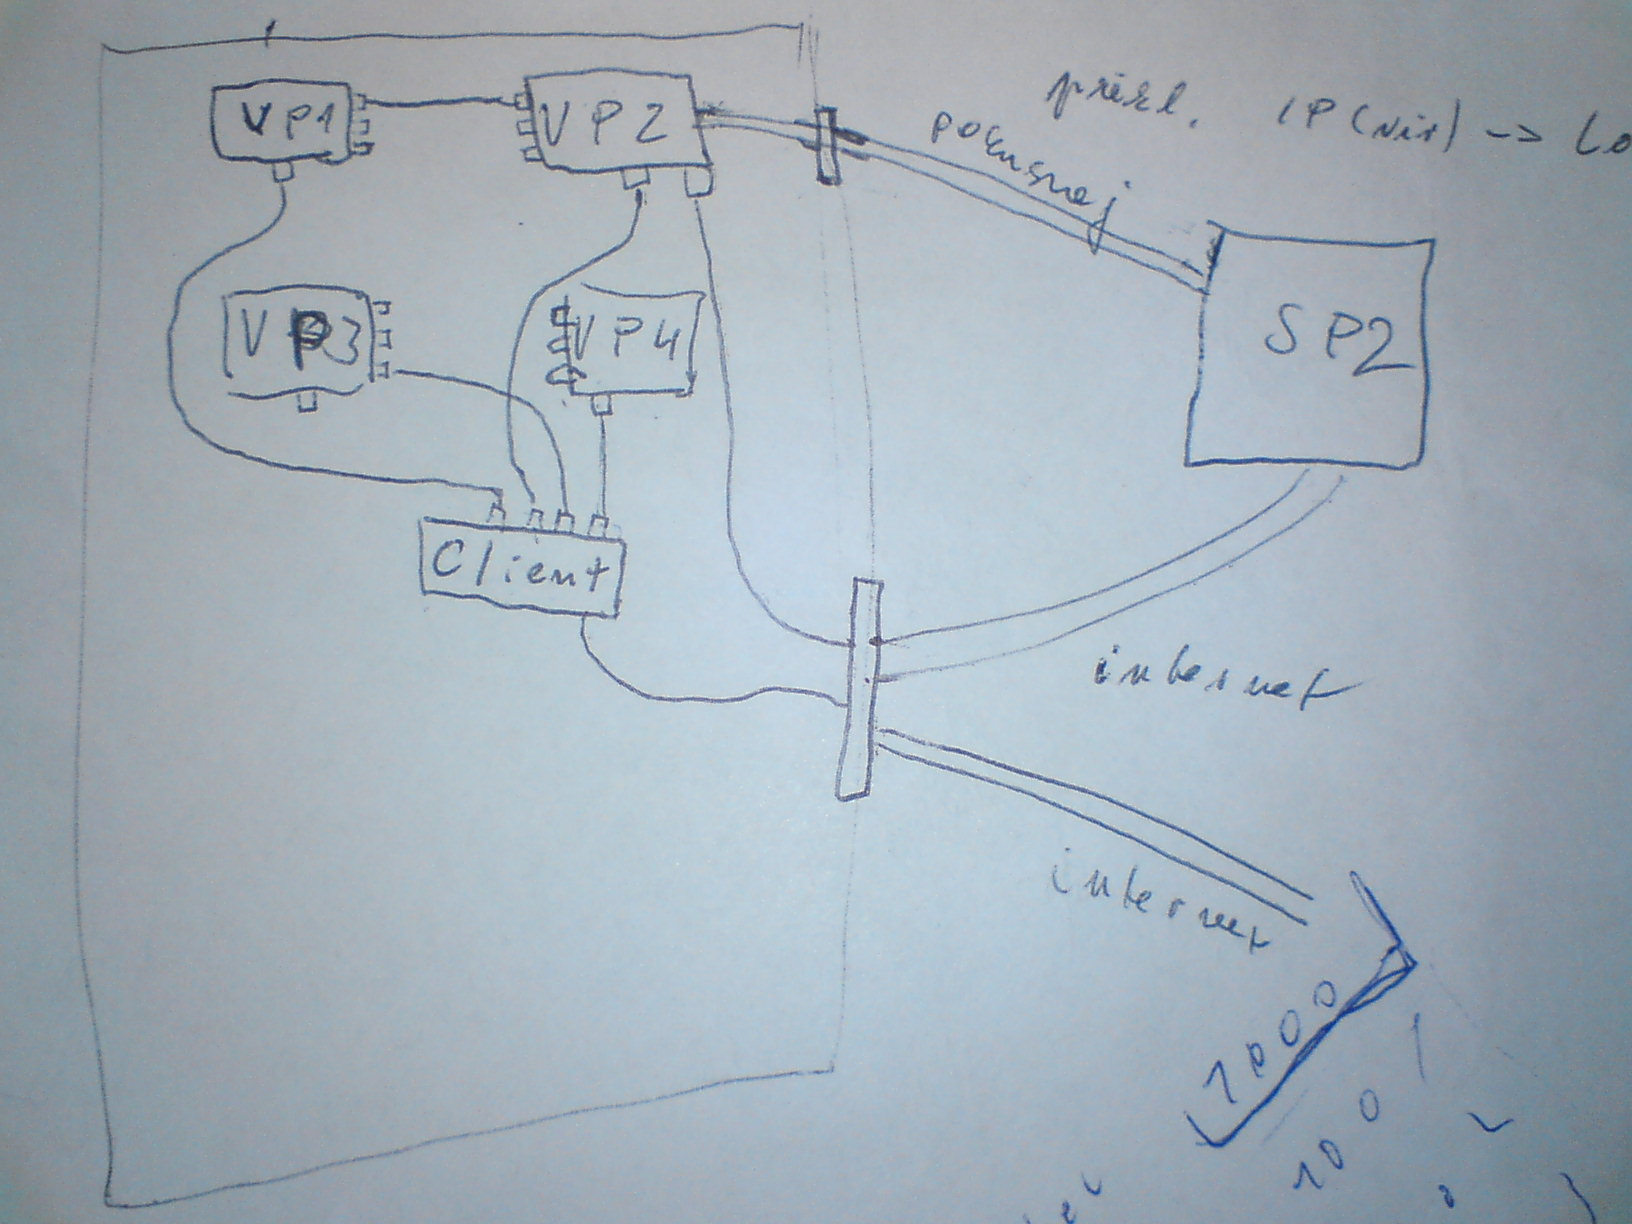
\includegraphics[width=9cm]{figures/navrh}
\caption{Počáteční návrh}
\label{fig:navrh}
\end{center}
\end{figure}

\subsection{Klient - server}\label{klien_server}
Síťovou vrstvu systému tvoří architektura klient - server. Ta, jak jsem již naznačoval v kapitole \ref{vymezeni}, byla převzata ze semestrální práce, kde bylo za úkol mimo jiné implementovat více-vláknový server. Server má sám pro sebe vlastní vlákno ve kterém běží. Dále server vytvoří při startu pro všechny počítače nová vlákna, která poslouchají na portu o jedna větším než předchozí počítač (první počítač začíná na portu předaným jako parametr při startu serveru). Tyto vlákna se chovají zase jako servery. Když se uživatel připojí na libovolný počítač, tak se vytvoří další vlákno pro obsluhu tohoto klienta. Výhodou tohoto řešení je, že je možné se připojit na kterýkoliv počítač kolikrát potřebujeme. Je to tedy přesně tak, jako bychom se připojovali na reálné Cisco či Linux např. přes protokol ssh\footnote{Secure Shell - zabezpečený komunikační protokol (v současné době náhrada telnetu)} či telnet.

\begin{figure}[h]
\begin{center}
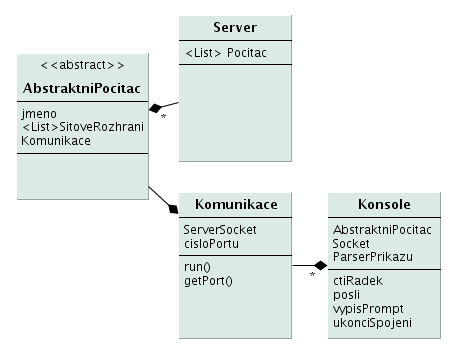
\includegraphics[width=9cm]{figures/uml_sit2}
\caption{Návrh komunikační části}
\label{fig:sit}
\end{center}
\end{figure}

Na obrázku \ref{fig:sit} je znázorněna komunikační část pomocí UML\footnote{Unified Modeling Language, UML je v softwarovém inženýrství grafický jazyk pro vizualizaci, specifikaci, navrhování a dokumentaci programových systémů.\cite{wiki:uml}} diagramu. Každý počítač má objekt \verb|Komunikace|, která čeká na připojení nového klienta. Když klient vyšle požadavek o nové spojení, tak se vytvoří \verb|Konsole|, která tohoto klienta bude obsluhovat. Při odpojení klienta \verb|Konsole| zaniká, protože její přítomnost už není potřeba.

\subsection{Vyhodnocování příkazů}
Když uživatel zadá příkaz a ukončí ho znakem nového řádku (klávesa Enter, znak \verb|\n|), tak se ve třídě \verb|Konzole| zavolá metoda \verb|zpracujRadek()|. Tuto metodu vlastní abstraktní \verb|ParserPrikazu|, který je v mém případe implementován jako \verb|CiscoParserPrikazu|\footnote{LinuxParser příkazů má na starosti kolega. Pro jiné typy počítačů je nutno implementovat parser vlastní.}. Ten se stará o zpracování poslané řádky a podle toho volá různé Cisco příkazy, které tvoří můj IOS, či jiné servisní příkazy.

% \newpage

\subsection{Datové struktury jádra}

Po architektuře klient - server bylo potřeba domyslet datové struktury virtuálních počítačů. Ze začátku jsem nastínil základní třídy a zbytek jsem dodělával jak bylo potřeba. 

\subsubsection{Směrovač - CiscoPocitac}
Na skutečné počítačové síti jsou síťové prvky několika druhů (switche, bridge, repeatery, směrovače, ..), ale na laboratorních cvičeních předmětu Y36PSI se  nastavují pouze směrovače ze 3. vrstvy\footnote{Tato \uv{síťová vrstva} se stará o směrování v síti a síťové adresování. Dále poskytuje spojení mezi vzdálenými sítěmi, které spolu přímo nesousedí.} síťového ISO/OSI modelu. Proto v mé práci figuruje pouze jeden typ síťového prvku - směrovač (router), který je reprezentován datovou strukturou \verb|CiscoPocitac| viz obrázek \ref{fig:class}. Ten je spojen přes vlastní rozhraní k jinému počítači přes jeho rozhraní právě jedním \uv{kabelem}. Není tedy možné, aby bylo jedno rozhraní připojeno k více rozhraním, protože jsou to všechno dvou bodové spoje. 

% \newpage

\begin{figure}[h]
\begin{center}
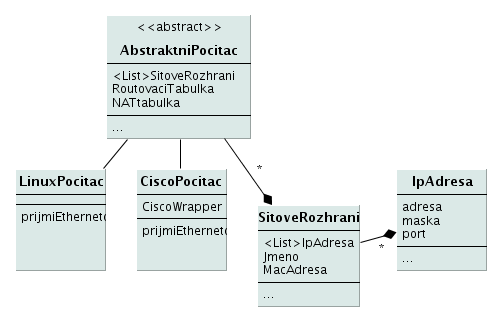
\includegraphics[width=10cm]{figures/uml_class}
\caption{Zjednodušený diagram tříd}
\label{fig:class}
\end{center}
\end{figure}

Nastavení propojení mezi počítači (respektive jejich rozhraními) je dáno v konfiguračním souboru. Původně každé rozhraní obsahovalo informaci, ke kterému rozhraní kterého počítače je připojeno. To se ale ukázalo jako zbytečně matoucí, protože informace o kabelu tam byla obsažena dvakrát. V dnešní verzi programu je to zjednodušené tak, že samotné rozhraní nenese žádnou informaci o kabelu. Ale kabely jsou konfiguračním souboru zvlášť:

\begin{verbatim}
<kabelaz>
  <kabel>
    <prvni>linux1:eth0</prvni>
    <druhy>linux2:eth0</druhy>
  </kabel>
  <kabel>
    <prvni>linux2:eth1</prvni>
    <druhy>cisco1:FastEthernet0/0</druhy>
  </kabel>
  <kabel>
    <prvni>cisco1:FastEthernet0/1</prvni>
    <druhy>cisco2:FastEthernet0/0</druhy>
  </kabel>
</kabelaz>
\end{verbatim} 

Konce kabelu jsou charakterizovány dvěma záznamy, každý obsahuje jméno počítače a rozhraní oddělené dvojtečkou.

% \newpage

\subsubsection{Síťové rozhraní}
Datová struktura pro síťové rozhraní je ve své podstatě jednoduchá. Obsahuje jméno, seznam IP adres přiřazených k tomuto rozhraní, MAC\footnote{MAC - Media Access Control, je fyzická adresa, kterou používá 2. (spojová) vrstva ISO/OSI modelu} adresu a stav.

Systémem je oficiálně podporována pouze jedna IP adresa per rozhraní, více adres si ale vyžádal překlad adres. MAC adresa je v tomto systému spíše pro větší přiblížení skutečnému rozhraní, protože ARP\footnote{Address Resolution Protocol se v počítačových sítích s IP protokolem používá k získání ethernetové MAC adresy sousedního stroje z jeho IP adresy. Používá se v situaci, kdy je třeba odeslat IP datagram na adresu ležící ve stejné podsíti jako odesilatel. Data se tedy mají poslat přímo adresátovi, u něhož však odesilatel zná pouze IP adresu. Pro odeslání prostřednictvím např. Ethernetu ale potřebuje znát cílovou ethernetovou adresu.\cite{wiki:arp}} protokol není u nás přímo implementován. Systém obsahuje pouze několik pravidel, které byly nutné pro rozhodování zda přijmout či nepřijmout příchozí paket. Dále rozhraní obsahuje indikátor stavu, ve kterém se nachází - zapnuté/vypnuté. Tento ukazatel jsem zavedl, protože rozhraní Cisca jsou ve výchozím stavu vypnutá.

\subsubsection{IP adresa}
IP adresa je mnohem složitější než rozhraní i když obsahuje pouze tři čísla reprezentující adresu, masku a port. Složitost je dána tím, že tato třída obsahuje přes 40 obslužných metod, které pokrývají veškerou práci, co je potřeba s adresou dělat.


\subsection{Telnet}
V zadání je přímo zmíněno použití programu telnet pro připojení klientů k serveru. Telnet je ale také protokol, po kterém se domlouvá telnet klient a telnet server. Česká wikipedie píše o telnet protokolu: \uv{Protokol přenáší osmibitové znaky oběma směry (duplexní spojení) a je velmi jednoduchý.\cite{wiki:telnet}}. Podle protokolu se vše posílá po znaku a protistrana po znaku vše potvrzuje. Protokol telnet ale zas tak jednoduchý není. Podporuje několik režimů, při navazování spojení začne proces vyjednávání atd. To všechno implementovat by bylo na samostatnou (možná i diplomovou) práci. 

Samotný telnet (ať protokol či program) ale neposkytuje doplňování příkazů nebo alespoň historii příkazů. Dalším problémem je, že při psaní příkazů přes telnet nefunguje editace aktuálního řádku, respektive lze mazat po znacích klávesou \verb|BackSpace|, ale nelze se pohybovat do stran šipkami doleva a doprava - při takovém pokusu to vypíše \verb|^[[D| či \verb|^[[C|. Tato \uv{vlastnost} se ale neprojevuje při připojování na vlastní telnet server. To je způsobeno tím, že v takovém případě se o editaci řádku a historii příkazů stará samotný BASH\footnote{Bourne again shell - nejpoužívanější unixový shell}. V případě této aplikace toho ale nelze využít, tak jsem se rozhodl, že tyto funkcionality budou na straně klienta, kde to bude zajišťovat \uv{někdo jiný}. 

Pro Linux jsem našel program rlwrap (readline wrapper), který přidává všechny tyto užitečné funkce: editace řádky, historie příkazů, doplňování příkazů, obarvení promptu. Pro Windows jsem nic takového nenašel, takže je to vyřešeno tak, že se vše pouští pod programem Cygwin. Navíc toto řešení zvyšuje komfort práce pod Windows, jelikož program \verb|cmd| není úplně uživatelsky přívětivý.


\section{Podobnost simulátoru se skutečným Ciscem}\label{kap:podobnost}
Při implementaci jsem se snažil vytvořit systém, který bude co nejvíce podobný skutečnému Ciscu. Musel jsem ale někde položit hranici mezi složitostí a věrností výsledné práce, protože tyto dvě metriky jsou vzájemném protikladu. Cisco IOS je natolik robustní a propracovaný systém, že je v mých silách pouze implementace úzké části systému, která je nutně potřeba pro splnění cíle. Byl jsem přinucen místy ustoupit a nechat vypsat hlášení, že to či ono není podporováno. V samotném parseru příkazů není toto téměř vůbec řešeno, protože by to znamenalo dopsání dohromady několika stovek pravidel pro všechny příkazy - např. příkaz \verb|ip| má 103 možností v konfiguračním stavu. Aby ale uživatel měl alespoň nějakou možnost se dopátrat, co je podporováno a co ne, tak jsem přidal příkaz \verb|help| (\verb|help_en| pro výpis v angličtině), který popisuje, co lze v jakém stavu Cisca použít.


\section{Programovací jazyk a prostředí}
Pro implementaci simulátoru jsem si vybral programovací jazyk Java hned z několika důvodů. Jazyk je to velmi robustní s bohatou sadou různých knihoven. Navíc programy vytvořené v tomto jazyce jsou zpravidla jednoduše přenositelné mezi různými operačními systémy, což je jeden z bodů nefunkčních požadavků. Jazyk Java disponuje propracovaným systémem výjimek, takže při nějaké neočekávané chybě se dozvíme víc, než v jazyce C++ s jeho \verb|Segmentation fault|. Neméně významným důvodem je i skutečnost, že s Javou mám zatím největší zkušenosti.

Celou práci jsem implementoval v Netbeans IDE\footnote{Integrated Development Environment} verze 6.8.


\section{Uživatelské rozhraní}
Uživatelské rozhraní je v zásadě velmi jednoduché. Vše je ovládáno přes příkazovou řádku, tak jak jsme zvyklí. Spuštění serveru je ulehčeno pomocným skriptem \verb|start_server.sh|, který zároveň obsahuje nápovědu. Pro připojování klientů jsem připravil skripty, ve kterých je zohledněna verze programu rlwrap. V balíčku programu Cygwin je rlwrap starší verze, která neumožňuje obarvování promptu a přeposílání signálů (např. při zmáčknutí Ctrl+C nebo Ctrl+Z). Novější verze už tyto funkce mají. Skripty pro připojení na \verb|linux.sh| a \verb|cisco.sh| fungují nezávisle na verzi.

\begin{figure}[h]
\begin{center}
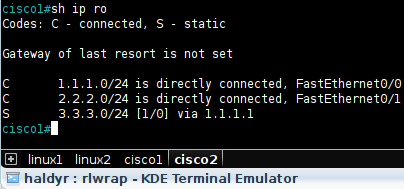
\includegraphics[height=2.5cm]{figures/uziv_rozhrani}
\caption{Uživatelské rozhraní pod OS Linux}
\label{fig:uziv_rozh}
\end{center}
\end{figure}

\section{Skutečné Cisco}
Jedním z největších \uv{oříšků} této práce bylo zjistit, jak se chová skutečné Cisco. Pravdou je, že Cisco Systems má na svých stránkách slušnou řadu návodů, nicméně není tak jednoduché v nich najít, co zrovna potřebujeme. A tak jsem hodně věcí zjišťoval z živého Cisca umístěného na Karlově náměstí přes protokol ssh. 









\chapter{Realizace}
Popis implementace/realizace se zaměřením na nestandardní části řešení.

A tady budu řešit jednotlivé Cisco příkazy - jak jsem na to přicházel, postupné problémy, moje implementace a odchylky.
% atd...

%*****************************************************************************

% Výsledná struktura vaší práce a~názvy a~rozsahy jednotlivých kapitol se samozřejmě budou lišit podle typu práce a~podle
% konkrétní povahy zpracovávaného tématu. Níže uvedená struktura práce odpovídá \textit{práci implementační}, viz
% \cite{infodp} respektive \cite{infobp}. 

%*****************************************************************************
\chapter{Testování}

\begin{itemize}
 \item Způsob, průběh a~výsledky testování.
 \item Srovnání s~existujícími řešeními, pokud jsou známy.
\end{itemize} 


%*****************************************************************************
\chapter{Závěr}
\section{Možnosti vylepšení}

\begin{itemize}
\item Zhodnocení splnění cílů DP/BP a~vlastního přínosu práce (při formulaci je třeba vzít v~potaz zadání práce).
\item Diskuse dalšího možného pokračování práce.
\begin{itemize}
\item graficke klikatko pro tvorbu XML konfiguraku
\item tcpdump
\item switche
\item napojeni na realnou sit
\item zpracovani signalu Ctrl+C, Ctrl+Z (-> vlastni klient, kouzlo telnetu je pak pryc)
\end{itemize} 


\end{itemize} 

%*****************************************************************************
% Seznam literatury je v samostatnem souboru reference.bib. Ten
% upravte dle vlastnich potreb, potom zpracujte (a do textu
% zapracujte) pomoci prikazu bibtex a nasledne pdflatex (nebo
% latex). Druhy z nich alespon 2x, aby se poresily odkazy.

% originally following specification for bibliography formating was used
%\bibliographystyle{abbrv}

% Here is an improvment by Petr Dlouhy (April 2010).
% It is mainly for supervisors who expect Czech fomrating rules for references
% Additional feature is live url addresses to sources from your pdf file
% It requires the file csplainnat.bst (included in this sample zipfile).

\bibliographystyle{csplainnat}

%bibliographystyle{plain}
%\bibliographystyle{psc}
{
%JZ: 11.12.2008 Kdo chce mit v techto ukazkovych odkazech take odkaz na CSTeX:
\def\CS{$\cal C\kern-0.1667em\lower.5ex\hbox{$\cal S$}\kern-0.075em $}
\bibliography{reference}
}

% M. Dušek radi:
%\bibliographystyle{alpha}
% kdy citace ma tvar [AutorRok] (napriklad [Cook97]). Sice to asi neni  podle ceske normy (BTW BibTeX stejne neodpovida
ceske norme), ale je to nejprehlednejsi.
% 3.5.2009 JZ polemizuje: BibTeX neobvinujte, napiste a poskytnete nam styl (.bst) splnujici citacni normu CSN/ISO.

%*****************************************************************************
%*****************************************************************************
\appendix

\chapter{Testování zaplnění stránky a~odsazení odstavců}
\textbf{\large Tato příloha nebude součástí vaší práce. 
Slouží pouze jako příklad formátování textu.}

\section*{}
Určitě existuje nějaká pěkná latinská věta, která se k~tomuhle testování používá, ale co mají dělat ti, kteří se nikdy
latinsky neučili? Určitě existuje nějaká pěkná latinská věta, která se k~tomuhle testování používá, ale co mají dělat
ti, kteří se nikdy latinsky neučili? Určitě existuje nějaká pěkná latinská věta, která se k~tomuhle testování používá,
ale co mají dělat ti, kteří se nikdy latinsky neučili?

Určitě existuje nějaká pěkná latinská věta, která se k~tomuhle testování používá, ale co mají dělat ti, kteří se nikdy
latinsky neučili? Určitě existuje nějaká pěkná latinská věta, která se k~tomuhle testování používá, ale co mají dělat
ti, kteří se nikdy latinsky neučili? Určitě existuje nějaká pěkná latinská věta, která se k~tomuhle testování používá,
ale co mají dělat ti, kteří se nikdy latinsky neučili?

Určitě existuje nějaká pěkná latinská věta, která se k~tomuhle testování používá, ale co mají dělat ti, kteří se nikdy
latinsky neučili? Určitě existuje nějaká pěkná latinská věta, která se k~tomuhle testování používá, ale co mají dělat
ti, kteří se nikdy latinsky neučili? Určitě existuje nějaká pěkná latinská věta, která se k~tomuhle testování používá,
ale co mají dělat ti, kteří se nikdy latinsky neučili?

Určitě existuje nějaká pěkná latinská věta, která se k~tomuhle testování používá, ale co mají dělat ti, kteří se nikdy
latinsky neučili? Určitě existuje nějaká pěkná latinská věta, která se k~tomuhle testování používá, ale co mají dělat
ti, kteří se nikdy latinsky neučili? Určitě existuje nějaká pěkná latinská věta, která se k~tomuhle testování používá,
ale co mají dělat ti, kteří se nikdy latinsky neučili? Určitě existuje nějaká pěkná latinská věta, která se k~tomuhle
testování používá, ale co mají dělat ti, kteří se nikdy latinsky neučili? Určitě existuje nějaká pěkná latinská věta,
která se k~tomuhle testování používá, ale co mají dělat ti, kteří se nikdy latinsky neučili? Určitě existuje nějaká
pěkná latinská věta, která se k~tomuhle testování používá, ale co mají dělat ti, kteří se nikdy latinsky neučili?

Určitě existuje nějaká pěkná latinská věta, která se k~tomuhle testování používá, ale co mají dělat ti, kteří se nikdy
latinsky neučili? Určitě existuje nějaká pěkná latinská věta, která se k~tomuhle testování používá, ale co mají dělat
ti, kteří se nikdy latinsky neučili?

Určitě existuje nějaká pěkná latinská věta, která se k~tomuhle testování používá, ale co mají dělat ti, kteří se nikdy
latinsky neučili? Určitě existuje nějaká pěkná latinská věta, která se k~tomuhle testování používá, ale co mají dělat
ti, kteří se nikdy latinsky neučili? Určitě existuje nějaká pěkná latinská věta, která se k~tomuhle testování používá,
ale co mají dělat ti, kteří se nikdy latinsky neučili? Určitě existuje nějaká pěkná latinská věta, která se k~tomuhle
testování používá, ale co mají dělat ti, kteří se nikdy latinsky neučili? Určitě existuje nějaká pěkná latinská věta,
která se k~tomuhle testování používá, ale co mají dělat ti, kteří se nikdy latinsky neučili?

Určitě existuje nějaká pěkná latinská věta, která se k~tomuhle testování používá, ale co mají dělat ti, kteří se nikdy
latinsky neučili? Určitě existuje nějaká pěkná latinská věta, která se k~tomuhle testování používá, ale co mají dělat
ti, kteří se nikdy latinsky neučili? Určitě existuje nějaká pěkná latinská věta, která se k~tomuhle testování používá,
ale co mají dělat ti, kteří se nikdy latinsky neučili? Určitě existuje nějaká pěkná latinská věta, která se k~tomuhle
testování používá, ale co mají dělat ti, kteří se nikdy latinsky neučili? Určitě existuje nějaká pěkná latinská věta,
která se k~tomuhle testování používá, ale co mají dělat ti, kteří se nikdy latinsky neučili?

Určitě existuje nějaká pěkná latinská věta, která se k~tomuhle testování používá, ale co mají dělat ti, kteří se nikdy
latinsky neučili? Určitě existuje nějaká pěkná latinská věta, která se k~tomuhle testování používá, ale co mají dělat
ti, kteří se nikdy latinsky neučili? Určitě existuje nějaká pěkná latinská věta, která se k~tomuhle testování používá,
ale co mají dělat ti, kteří se nikdy latinsky neučili? Určitě existuje nějaká pěkná latinská věta, která se k~tomuhle
testování používá, ale co mají dělat ti, kteří se nikdy latinsky neučili? Určitě existuje nějaká pěkná latinská věta,
která se k~tomuhle testování používá, ale co mají dělat ti, kteří se nikdy latinsky neučili?

Určitě existuje nějaká pěkná latinská věta, která se k~tomuhle testování používá, ale co mají dělat ti, kteří se nikdy
latinsky neučili? Určitě existuje nějaká pěkná latinská věta, která se k~tomuhle testování používá, ale co mají dělat
ti, kteří se nikdy latinsky neučili? Určitě existuje nějaká pěkná latinská věta, která se k~tomuhle testování používá,
ale co mají dělat ti, kteří se nikdy latinsky neučili? Určitě existuje nějaká pěkná latinská věta, která se k~tomuhle
testování používá, ale co mají dělat ti, kteří se nikdy latinsky neučili? Určitě existuje nějaká pěkná latinská věta,
která se k~tomuhle testování používá, ale co mají dělat ti, kteří se nikdy latinsky neučili?

Určitě existuje nějaká pěkná latinská věta, která se k~tomuhle testování používá, ale co mají dělat ti, kteří se nikdy
latinsky neučili? Určitě existuje nějaká pěkná latinská věta, která se k~tomuhle testování používá, ale co mají dělat
ti, kteří se nikdy latinsky neučili? Určitě existuje nějaká pěkná latinská věta, která se k~tomuhle testování používá,
ale co mají dělat ti, kteří se nikdy latinsky neučili? Určitě existuje nějaká pěkná latinská věta, která se k~tomuhle
testování používá, ale co mají dělat ti, kteří se nikdy latinsky neučili? Určitě existuje nějaká pěkná latinská věta,
která se k~tomuhle testování používá, ale co mají dělat ti, kteří se nikdy latinsky neučili?

Určitě existuje nějaká pěkná latinská věta, která se k~tomuhle testování používá, ale co mají dělat ti, kteří se nikdy
latinsky neučili? Určitě existuje nějaká pěkná latinská věta, která se k~tomuhle testování používá, ale co mají dělat
ti, kteří se nikdy latinsky neučili? Určitě existuje nějaká pěkná latinská věta, která se k~tomuhle testování používá,
ale co mají dělat ti, kteří se nikdy latinsky neučili? Určitě existuje nějaká pěkná latinská věta, která se k~tomuhle
testování používá, ale co mají dělat ti, kteří se nikdy latinsky neučili? Určitě existuje nějaká pěkná latinská věta,
která se k~tomuhle testování používá, ale co mají dělat ti, kteří se nikdy latinsky neučili?

Určitě existuje nějaká pěkná latinská věta, která se k~tomuhle testování používá, ale co mají dělat ti, kteří se nikdy
latinsky neučili? Určitě existuje nějaká pěkná latinská věta, která se k~tomuhle testování používá, ale co mají dělat
ti, kteří se nikdy latinsky neučili? Určitě existuje nějaká pěkná latinská věta, která se k~tomuhle testování používá,
ale co mají dělat ti, kteří se nikdy latinsky neučili? Určitě existuje nějaká pěkná latinská věta, která se k~tomuhle
testování používá, ale co mají dělat ti, kteří se nikdy latinsky neučili? Určitě existuje nějaká pěkná latinská věta,
která se k~tomuhle testování používá, ale co mají dělat ti, kteří se nikdy latinsky neučili?

Určitě existuje nějaká pěkná latinská věta, která se k~tomuhle testování používá, ale co mají dělat ti, kteří se nikdy
latinsky neučili? Určitě existuje nějaká pěkná latinská věta, která se k~tomuhle testování používá, ale co mají dělat
ti, kteří se nikdy latinsky neučili? Určitě existuje nějaká pěkná latinská věta, která se k~tomuhle testování používá,
ale co mají dělat ti, kteří se nikdy latinsky neučili? Určitě existuje nějaká pěkná latinská věta, která se k~tomuhle
testování používá, ale co mají dělat ti, kteří se nikdy latinsky neučili? Určitě existuje nějaká pěkná latinská věta,
která se k~tomuhle testování používá, ale co mají dělat ti, kteří se nikdy latinsky neučili?

Určitě existuje nějaká pěkná latinská věta, která se k~tomuhle testování používá, ale co mají dělat ti, kteří se nikdy
latinsky neučili? Určitě existuje nějaká pěkná latinská věta, která se k~tomuhle testování používá, ale co mají dělat
ti, kteří se nikdy latinsky neučili? Určitě existuje nějaká pěkná latinská věta, která se k~tomuhle testování používá,
ale co mají dělat ti, kteří se nikdy latinsky neučili? Určitě existuje nějaká pěkná latinská věta, která se k~tomuhle
testování používá, ale co mají dělat ti, kteří se nikdy latinsky neučili? Určitě existuje nějaká pěkná latinská věta,
která se k~tomuhle testování používá, ale co mají dělat ti, kteří se nikdy latinsky neučili?

Určitě existuje nějaká pěkná latinská věta, která se k~tomuhle testování používá, ale co mají dělat ti, kteří se nikdy
latinsky neučili? Určitě existuje nějaká pěkná latinská věta, která se k~tomuhle testování používá, ale co mají dělat
ti, kteří se nikdy latinsky neučili? Určitě existuje nějaká pěkná latinská věta, která se k~tomuhle testování používá,
ale co mají dělat ti, kteří se nikdy latinsky neučili? Určitě existuje nějaká pěkná latinská věta, která se k~tomuhle
testování používá, ale co mají dělat ti, kteří se nikdy latinsky neučili? Určitě existuje nějaká pěkná latinská věta,
která se k~tomuhle testování používá, ale co mají dělat ti, kteří se nikdy latinsky neučili?

Určitě existuje nějaká pěkná latinská věta, která se k~tomuhle testování používá, ale co mají dělat ti, kteří se nikdy
latinsky neučili? Určitě existuje nějaká pěkná latinská věta, která se k~tomuhle testování používá, ale co mají dělat
ti, kteří se nikdy latinsky neučili? Určitě existuje nějaká pěkná latinská věta, která se k~tomuhle testování používá,
ale co mají dělat ti, kteří se nikdy latinsky neučili? Určitě existuje nějaká pěkná latinská věta, která se k~tomuhle
testování používá, ale co mají dělat ti, kteří se nikdy latinsky neučili? Určitě existuje nějaká pěkná latinská věta,
která se k~tomuhle testování používá, ale co mají dělat ti, kteří se nikdy latinsky neučili?

Určitě existuje nějaká pěkná latinská věta, která se k~tomuhle testování používá, ale co mají dělat ti, kteří se nikdy
latinsky neučili? Určitě existuje nějaká pěkná latinská věta, která se k~tomuhle testování používá, ale co mají dělat
ti, kteří se nikdy latinsky neučili? Určitě existuje nějaká pěkná latinská věta, která se k~tomuhle testování používá,
ale co mají dělat ti, kteří se nikdy latinsky neučili? Určitě existuje nějaká pěkná latinská věta, která se k~tomuhle
testování používá, ale co mají dělat ti, kteří se nikdy latinsky neučili? Určitě existuje nějaká pěkná latinská věta,
která se k~tomuhle testování používá, ale co mají dělat ti, kteří se nikdy latinsky neučili?

Určitě existuje nějaká pěkná latinská věta, která se k~tomuhle testování používá, ale co mají dělat ti, kteří se nikdy
latinsky neučili? Určitě existuje nějaká pěkná latinská věta, která se k~tomuhle testování používá, ale co mají dělat
ti, kteří se nikdy latinsky neučili? Určitě existuje nějaká pěkná latinská věta, která se k~tomuhle testování používá,
ale co mají dělat ti, kteří se nikdy latinsky neučili? Určitě existuje nějaká pěkná latinská věta, která se k~tomuhle
testování používá, ale co mají dělat ti, kteří se nikdy latinsky neučili? Určitě existuje nějaká pěkná latinská věta,
která se k~tomuhle testování používá, ale co mají dělat ti, kteří se nikdy latinsky neučili?

Určitě existuje nějaká pěkná latinská věta, která se k~tomuhle testování používá, ale co mají dělat ti, kteří se nikdy
latinsky neučili? Určitě existuje nějaká pěkná latinská věta, která se k~tomuhle testování používá, ale co mají dělat
ti, kteří se nikdy latinsky neučili? Určitě existuje nějaká pěkná latinská věta, která se k~tomuhle testování používá,
ale co mají dělat ti, kteří se nikdy latinsky neučili? Určitě existuje nějaká pěkná latinská věta, která se k~tomuhle
testování používá, ale co mají dělat ti, kteří se nikdy latinsky neučili? Určitě existuje nějaká pěkná latinská věta,
která se k~tomuhle testování používá, ale co mají dělat ti, kteří se nikdy latinsky neučili?

Určitě existuje nějaká pěkná latinská věta, která se k~tomuhle testování používá, ale co mají dělat ti, kteří se nikdy
latinsky neučili? Určitě existuje nějaká pěkná latinská věta, která se k~tomuhle testování používá, ale co mají dělat
ti, kteří se nikdy latinsky neučili? Určitě existuje nějaká pěkná latinská věta, která se k~tomuhle testování používá,
ale co mají dělat ti, kteří se nikdy latinsky neučili? Určitě existuje nějaká pěkná latinská věta, která se k~tomuhle
testování používá, ale co mají dělat ti, kteří se nikdy latinsky neučili? Určitě existuje nějaká pěkná latinská věta,
která se k~tomuhle testování používá, ale co mají dělat ti, kteří se nikdy latinsky neučili?

%*****************************************************************************

\chapter{Pokyny a~návody k~formátování textu práce}
\textbf{\large Tato příloha samozřejmě nebude součástí vaší práce. Slouží pouze jako příklad formátování textu.}

Používat se dají všechny příkazy systému \LaTeX. Existuje velké množství volně přístupné dokumentace, tutoriálů,
příruček a~dalších materiálů v~elektronické podobě. Výchozím bodem, kromě Googlu, může být stránka CSTUG (Czech Tech
Users Group) \cite{CSTUG}. Tam najdete odkazy na další materiály.  Vetšinou dostačující a~přehledně organizovanou
elektronikou dokumentaci najdete například na \cite{latexdocweb} nebo \cite{latexwiki}.

Existují i~různé nadstavby nad systémy \TeX{} a~\LaTeX, které výrazně usnadní psaní textu zejména začátečníkům. Velmi
rozšířený v~Linuxovém prostředí je systém Kile.


\section{Vkládání obrázků}
Obrázky se umísťují do plovoucího prostředí \verb|figure|. Každý obrázek by měl obsahovat \textbf{název}
(\verb|\caption|) a~\textbf{návěští} (\verb|\label|). Použití příkazu pro vložení obrázku \\\verb|\includegraphics| je
podmíněno aktivací (načtením) balíku graphicx příkazem\\ \verb|\usepackage{graphicx}|.

Budete-li zdrojový text zpracovávat pomocí programu \verb|pdflatex|, očekávají se obrázky s~příponou
\verb|*.pdf|\footnote{pdflatex umí také formáty PNG a~JPG.}, použijete-li k~formátování \verb|latex|, očekávají se
obrázky s~příponou \verb|*.eps|.\footnote{Vzájemnou konverzi mezi snad všemi typy obrazku včetně změn vekostí a~dalších
vymožeností vám může zajistit balík ImageMagic  (http://www.imagemagick.org/script/index.php). Je dostupný pod Linuxem,
Mac OS i~MS Windows. Důležité jsou zejména příkazy convert a~identify.}


\begin{figure}[ht]
\begin{center}

\includegraphics[width=5cm]{figures/LogoCVUT}
\caption{Popiska obrázku}
\label{fig:logo}
\end{center}
\end{figure}

Příklad vložení obrázku:
\begin{verbatim}
\begin{figure}[h]
\begin{center}

\includegraphics[width=5cm]{figures/LogoCVUT}
\caption{Popiska obrazku}
\label{fig:logo}
\end{center}
\end{figure}
\end{verbatim}

\section{Kreslení obrázků}
Zřejmě každý z~vás má nějaký oblíbený nástroj pro tvorbu obrázků. Jde jen o~to, abyste dokázali obrázek uložit
v~požadovaném formátu nebo jej do něj konvertovat (viz předchozí kapitola). Je zřejmě vhodné kreslit obrázky vektorově.
Celkem oblíbený, na ovládání celkem jednoduchý a~přitom dostatečně mocný je například program Inkscape.

Zde stojí za to upozornit na kreslící programe Ipe \cite{ipe}, který dokáže do obrázku vkládat komentáře přímo
v~latexovském formátu (vzroce, stejné fonty atd.). Podobné věci umí na Linuxové platformě nástroj Xfig. 

Za pozornost ještě stojí schopnost editoru Ipe importovat obrázek (jpg nebo bitmap) a~krelit do něj latexovské popisky
a~komentáře. Výsledek pak umí exportovat přímo do pdf.


\section{Tabulky}
Existuje více způsobů, jak sázet tabulky. Například je možno použít prostředí \verb|table|, které je velmi podobné
prostředí \verb|figure|. 

\begin{table}
\begin{center}
\begin{tabular}{|c|l|l|}
\hline
\textbf{DTD} & \textbf{construction} & \textbf{elimination} \\
\hline
$\mid$ & \verb+in1|A|B a:sum A B+ & \verb+case([_:A]a)([_:B]a)ab:A+\\
&\verb+in1|A|B b:sum A B+ & \verb+case([_:A]b)([_:B]b)ba:B+\\
\hline
$+$&\verb+do_reg:A -> reg A+&\verb+undo_reg:reg A -> A+\\
\hline
$*,?$& the same like $\mid$ and $+$ & the same like $\mid$ and $+$\\
& with \verb+emtpy_el:empty+ & with \verb+emtpy_el:empty+\\
\hline
R(a,b) & \verb+make_R:A->B->R+ & \verb+a: R -> A+\\
 & & \verb+b: R -> B+\\
\hline
\end{tabular}
\end{center}
\caption{Ukázka tabulky}
\label{tab:tab1}
\end{table}

Zdrojový text tabulky \ref{tab:tab1} vypadá takto:
\begin{verbatim}
\begin{table}
\begin{center}
\begin{tabular}{|c|l|l|}
\hline
\textbf{DTD} & \textbf{construction} & \textbf{elimination} \\
\hline
$\mid$ & \verb+in1|A|B a:sum A B+ & \verb+case([_:A]a)([_:B]a)ab:A+\\
&\verb+in1|A|B b:sum A B+ & \verb+case([_:A]b)([_:B]b)ba:B+\\
\hline
$+$&\verb+do_reg:A -> reg A+&\verb+undo_reg:reg A -> A+\\
\hline
$*,?$& the same like $\mid$ and $+$ & the same like $\mid$ and $+$\\
& with \verb+emtpy_el:empty+ & with \verb+emtpy_el:empty+\\
\hline
R(a,b) & \verb+make_R:A->B->R+ & \verb+a: R -> A+\\
 & & \verb+b: R -> B+\\
\hline
\end{tabular}
\end{center}
\caption{Ukázka tabulky}
\label{tab:tab1}
\end{table}
\begin{table}
\end{verbatim}

\section{Odkazy v~textu}
\subsection{Odkazy na literaturu}
Jsou realizovány příkazem \verb|\cite{odkaz}|. 

Seznam literatury je dobré zapsat do samostatného souboru a~ten pak zpracovat programem bibtex (viz soubor
\verb|reference.bib|). Zdrojový soubor pro \verb|bibtex| vypadá například takto:
\begin{verbatim}
@Article{Chen01,
  author  = "Yong-Sheng Chen and Yi-Ping Hung and Chiou-Shann Fuh",
  title   = "Fast Block Matching Algorithm Based on 
             the Winner-Update Strategy",
  journal = "IEEE Transactions On Image Processing",
  pages   = "1212--1222",
  volume  =  10,
  number  =   8,
  year    = 2001,
}

@Misc{latexdocweb,
  author  = "",
  title   = "{\LaTeX} --- online manuál",
  note    = "\verb|http://www.cstug.cz/latex/lm/frames.html|",
  year    = "",
}
...
\end{verbatim}

%11.12.2008, 3.5.2009
\textbf{Pozor:} Sazba názvů odkazů je dána Bib\TeX{} stylem\\ (\verb|\bibliographystyle{abbrv}|). 
%Budete-li používat české prostředí (\verb|\usepackage[czech]{babel}|), 
Bib\TeX{} tedy obvykle vysází velké pouze počáteční písmeno z~názvu zdroje, 
ostatní písmena zůstanou malá bez ohledu na to, jak je napíšete. 
Přesněji řečeno, styl může zvolit pro každý typ publikace jiné konverze. 
Pro časopisecké články třeba výše uvedené, jiné pro monografie (u~nich často bývá 
naopak velikost písmen zachována).

Pokud chcete Bib\TeX u napovědět, která písmena nechat bez konverzí 
(viz \texttt{title = "\{$\backslash$LaTeX\} -{}-{}- online manuál"} 
v~předchozím příkladu), je nutné příslušné písmeno (zde celé makro) uzavřít 
do složených závorek. Pro přehlednost je proto vhodné celé parametry 
uzavírat do uvozovek (\texttt{author = "\dots"}), nikoliv do složených závorek.

Odkazy na literaturu ve zdrojovém textu se pak zapisují:
\begin{verbatim}
Podívejte se na \cite{Chen01}, 
další detaily najdete na \cite{latexdocweb}
\end{verbatim}

Vazbu mezi soubory \verb|*.tex| a~\verb|*.bib| zajistíte příkazem 
\verb|\bibliography{}| v~souboru \verb|*.tex|.  V~našem případě tedy zdrojový 
dokument \verb|thesis.tex| obsahuje příkaz\\
\verb|\bibliography{reference}|.

Zpracování zdrojového textu s~odkazy se provede postupným voláním programů\\
\verb|pdflatex <soubor>| (případně \verb|latex <soubor>|), \verb|bibtex <soubor>| 
a~opět\\ \verb|pdflatex <soubor>|.\footnote{První volání \texttt{pdflatex} 
vytvoří soubor s~koncovkou \texttt{*.aux}, který je vstupem pro program 
\texttt{bibtex}, pak je potřeba znovu zavolat program \texttt{pdflatex} 
(\texttt{latex}), který tentokrát zpracuje soubory s~příponami \texttt{.aux}
a~\texttt{.tex}. 
Informaci o~případných nevyřešených odkazech (cross-reference) vidíte přímo při 
zpracovávání zdrojového souboru příkazem \texttt{pdflatex}. Program \texttt{pdflatex} 
(\texttt{latex}) lze volat vícekrát, pokud stále vidíte nevyřešené závislosti.}


Níže uvedený příklad je převzat z~dříve existujících pokynů studentům, kteří 
dělají svou diplomovou nebo bakalářskou práci v~Grafické skupině.\footnote{Několikrát 
jsem byl upozorněn, že web s~těmito pokyny byl zrušen, proto jej zde přímo necituji. 
Nicméně příklad sám o~sobě dokumentuje obecně přijímaný konsensus ohledně citací 
v~bakalářských a~diplomových pracích na KP.} Zde se praví:
\begin{small}
\begin{verbatim}
...
j) Seznam literatury a dalších použitých pramenů, odkazy na WWW stránky, ...
 Pozor na to, že na veškeré uvedené prameny se musíte v textu práce 
 odkazovat -- [1]. 
Pramen, na který neodkazujete, vypadá, že jste ho vlastně nepotřebovali 
a je uveden jen do počtu. Příklad citace knihy [1], článku v časopise [2], 
stati ve sborníku [3] a html odkazu [4]: 
[1] J. Žára, B. Beneš;, and P. Felkel. 
     Moderní počítačová grafika. Computer Press s.r.o, Brno, 1 edition, 1998. 
     (in Czech). 
[2] P. Slavík. Grammars and Rewriting Systems as Models for Graphical User 
     Interfaces. Cognitive Systems, 4(4--3):381--399, 1997. 
[3] M. Haindl, Š. Kment, and P. Slavík. Virtual Information Systems. 
     In WSCG'2000 -- Short communication papers, pages 22--27, Pilsen, 2000. 
     University of West Bohemia. 
[4] Knihovna grafické skupiny katedry počítačů: 
     http://www.cgg.cvut.cz/Bib/library/ 
\end{verbatim}
\end{small}
\ldots{} abychom výše citované odkazy skutečně našli v~(automaticky generovaném) seznamu literatury tohoto textu, musíme
je nyní alespoň jednou citovat: Kniha \cite{kniha}, článek v~časopisu \cite{clanek}, příspěvek na konferenci
\cite{sbornik}, www odkaz \cite{www}.

Ještě přidáme další ukázku citací online zdrojů podle české normy. Odkaz na wiki o~frameworcich \cite{wiki:framework}
a~ORM \cite{wiki:orm}. Použití viz soubor \verb|reference.bib|. V~seznamu literatury by nyní měly být živé odkazy na
zdroje. V~\verb|reference.bib| je zcela nový typ publikace. Detaily dohledal a~dodal Petr Dlouhý v~dubnu 2010.
Podrobnosti najdete ve zdrojovém souboru tohoto textu v~komentáři u~příkazu \verb|\thebibliography|.

\subsection{Odkazy na obrázky, tabulky a~kapitoly}
\begin{itemize}
\item Označení místa v~textu, na které chcete později čtenáře práce odkázat, se provede příkazem \verb|\label{navesti}|.
Lze použít v~prostředích \verb|figure| a~\verb|table|, ale též za názvem kapitoly nebo podkapitoly.
\item Na návěští se odkážeme příkazem \verb|\ref{navesti}| nebo \verb|\pageref{navesti}|.
\end{itemize}

\section{Rovnice, centrovaná, číslovaná matematika}
Jednoduchý matematický výraz zapsaný přímo do textu se vysází pomocí prostředí \verb|math|, resp. zkrácený zápis pomocí
uzavření textu rovnice mezi znaky \verb|$|.

Kód \verb|$ S = \pi * r^2 $| bude vysázen takto: $ S = \pi * r^2 $.

Pokud chcete nečíslované rovnice, ale umístěné centrovaně na samostatné řádky, pak lze použít prostředí
\verb|displaymath|, resp. zkrácený zápis pomocí uzavření textu rovnice mezi znaky \verb|$$|. Zdrojový kód: 
\begin{verb}
|$$ S = \pi * r^2 $$|
\end{verb}
bude pak vysázen takto:
$$ S = \pi * r^2 $$

Chcete-li mít rovnice číslované, je třeba použít prostředí \verb|eqation|. Kód:
\begin{verbatim}
\begin{equation}
  S = \pi * r^2
\end{equation}

\begin{equation}
  V = \pi * r^3
\end{equation}
\end{verbatim}
je potom vysázen takto:
\begin{equation}
  S = \pi * r^2
\end{equation}

\begin{equation}
  V = \pi * r^3
\end{equation}

\section{Kódy programu}
Chceme-li vysázet například část zdrojového kódu programu (bez formátování), hodí se prostředí \verb|verbatim|: 
\begin{verbatim}
         (* nickname2 *)
Lego> Refine in1
             (do_reg (nickname1 h));
Refine by  in1 (do_reg (nickname1 h))
   ?4 : pcdata
   ?5 : pcdata
          (* surname2 *)
Lego> Refine surname1 h;
Refine by  surname1 h
   ?5 : pcdata
          (* email2 *)
Lego> Refine undo_reg (email1 h);
Refine by  undo_reg (email1 h)
*** QED ***
\end{verbatim}

\section{Další poznámky}
\subsection{České uvozovky}
V~souboru \verb|k336_thesis_macros.tex| je příkaz \verb|\uv{}| pro sázení českých uvozovek. \uv{Text uzavřený do českých
uvozovek.}

% JZ: 3.5.2009 \chapter z book zajistí automaticky
%\subsection{Začátky kapitol na liché stránky}
%Ve výsledném textu je dobré, když každá kapitola začíná na liché stránce. Tedy použijte:
%\begin{verbatim}
%  \cleardoublepage\chapter{Úvod} \label{uvod}

% Úvod charakterizující kontext zadání, případně motivace.
% ----------
% Navrhněte a~implementujte aplikaci, která umožní vytvoření virtuální počítačové sítě, pro potřeby předmětu Y36PSI. Na
% systém se bude možno připojit s~pomocí telnetu. Z~pohledu uživatele se bude systém tvářit jako reálná síť. Zaměřte se
% především na konfiguraci systému Cisco. Systém bude podporovat příkazy potřebné ke konfiguraci síťových rozhraní,
% směrování a~překladu adres. Pro ověření správnosti konfigurace implementujte příkaz ping a~traceroute.

Úkolem této práce je navrhnout a implementovat aplikaci, která umožní vytvoření virtuální počítačové sítě pro předmět Y36PSI Počítačové sítě. Z pohledu uživatele se systém musí tvářit jako reálná síť. Tento úkol byl rozdělen na dvě části: Cisco a Linux. Můj úkol je právě emulace Cisco IOS\footnote{Internetwork Operating System je operační systém používaný na směrovačích a přepínačích firmy Cisco Systems}. Na dnešním virtuálním trhu existuje celá řada programů pro virtualizaci sítě. Většina z nich je však špatně dostupných (zejména kvůli licenci) nebo se nehodí pro potřeby předmětu Počítačové sítě. 

Vize je taková, že student si v teple domova spustí tuto aplikaci a \uv{pohraje} si s virtuálním ciscem, ke kterému běžný smrtelník nemá přístup. Zjistí, jak to funguje a pak už jen přijde na cvičení předmětu a vše nakonfiguruje tak, jak to má být. 

Tato práce je v rozsahu týmového projektu, protože přesahuje rozsah jedné bakalářské práce. Byly vymezeny hranice, aby se tento úkol mohl rozdělit na dvě části. Nakonec celá aplikace byla rozdělena na tři části. První je část společná, kde je implementováno jádro klient - server. Druhá část je Cisco IOS, tu jsem implementoval já. A třetí část je platforma Linux, kterou zpracoval Tomáš Pitřinec v bakalářské práci Simulátor virtuální počítačové sítě Linux.

\section{Struktura práce}
Tady bude popis členění práce na jednotivé sekce.
%  \cleardoublepage\include{2_teorie}
%   atd.\ldots{}
%\end{verbatim}

%*****************************************************************************
\chapter{Seznam použitých zkratek}

\begin{description}
\item[CLI] Command Line Interface
\item[IOS] Internetwork Operating System
\item[NAT] Network Address Translation
\item[Y36PSI] předmět Počítačové sítě
\end{description}
\vdots

%*****************************************************************************
\chapter{UML diagramy}
\textbf{\large Tato příloha není povinná a~zřejmě se neobjeví v~každé práci. Máte-li ale větší množství podobných
diagramů popisujících systém, není nutné všechny umísťovat do hlavního textu, zvláště pokud by to snižovalo jeho
čitelnost.}

%*****************************************************************************
\chapter{Instalační a~uživatelská příručka}
\textbf{\large Tato příloha velmi žádoucí zejména u~softwarových implementačních prací.}

%*****************************************************************************
\chapter{Obsah přiloženého CD}
\textbf{\large Tato příloha je povinná pro každou práci. Každá práce musí totiž obsahovat přiložené CD. Viz dále.}

Může vypadat například takto. Váš seznam samozřejmě bude odpovídat typu vaší práce. (viz \cite{infodp}):

\begin{figure}[h]
\begin{center}
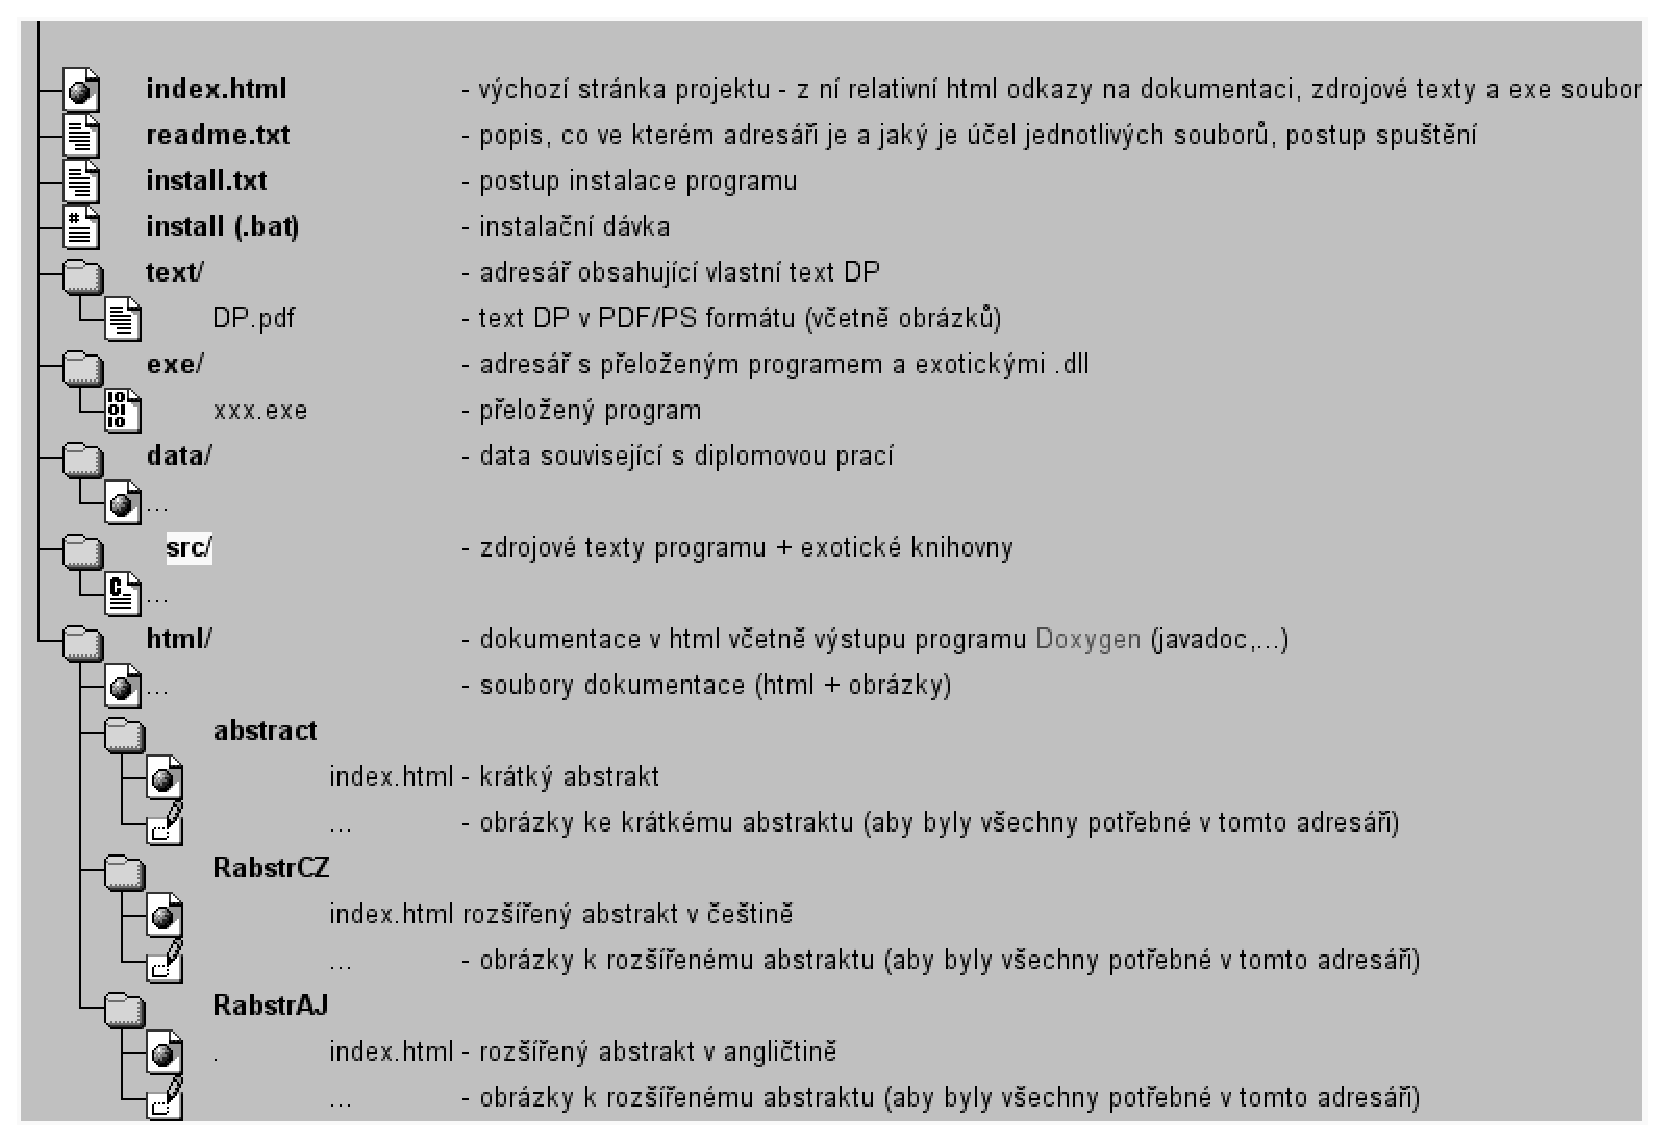
\includegraphics[width=14cm]{figures/seznamcd}
\caption{Seznam přiloženého CD --- příklad}
\label{fig:seznamcd}
\end{center}
\end{figure}

Na GNU/Linuxu si strukturu přiloženého CD můžete snadno vyrobit příkazem:\\ 
\verb|$ tree . >tree.txt|\\
Ve vzniklém souboru pak stačí pouze doplnit komentáře.

Z~\textbf{README.TXT} (případne index.html apod.)  musí být rovněž zřejmé, jak programy instalovat, spouštět a~jaké
požadavky mají tyto programy na hardware.

Adresář \textbf{text}  musí obsahovat soubor s~vlastním textem práce v~PDF nebo PS formátu, který bude později použit
pro prezentaci diplomové práce na WWW.

\end{document}
